\chapter{Large-Scale Toxicity Analysis Pipeline} \label{large-scale-pipeline}
This chapter describes the technical workflow for processing and analyzing toxicity in social media posts, specifically focusing on English-language toots from Mastodon instances. The pipeline is built using the Ray framework \cite{moritz:2018}, which enables distributed computing for efficient large-scale data processing. The pipeline consists of several stages: data reading, deduplication, toxicity prediction, and merging. Each stage is designed to handle large datasets efficiently, leveraging parallel processing and optimized memory usage.

\paragraph{Prerequisites}
The Ray environment is configured with specific settings to ensure efficient processing of large datasets.
\todo[inline]{describe the parameters used in \textit{map\_batches} to get a good perforamce on our cluster}
To ensure robustness, the pipeline is configured to retry failed tasks up to 10 times, with retry exceptions enabled to handle transient errors gracefully.

These settings ensure that the pipeline can handle large datasets efficiently on our cluster while minimizing resource contention. The use of \textit{map\_batches} in the pandas format allows for seamless integration with data processing functions, enabling parallel execution of tasks.

\section{Reading and Processing Toots}\label{step:ingestion} 
The pipeline's first stage retrieves Mastodon data from Elasticsearch using the following filters:

\begin{enumerate}
    \item \textbf{Temporal scope}: Only toots posted during 2024
    \item \textbf{Instance selection}: From 1,000 fully crawled instances
    \item \textbf{Content filters}:
    \begin{itemize}
        \item Original toots only (excluding reblogs/boosts)
        \item Text-only content (removing toots with media attachments)
        \item English-language labeled content
    \end{itemize}
\end{enumerate}

We use the \textit{ray\_elasticsearch}\footnote{\url{https://github.com/janheinrichmerker/ray-elasticsearch}} library for efficient Elasticsearch queries. The retrieved data contains the fields described in Table~\ref{dataset-fields}, including toot identifiers, content, instance information, and metadata flags. To avoid overloading the Elasticsearch cluster, we read data directly into local storage using the Parquet\footnote{\url{https://github.com/apache/parquet-java}} file format for efficient storage.

For our toxicity analysis, we use a 10\% subsample of the dataset due to time constraints. To obtain the subsample we apply the \textit{sample} method from the pandas library before further processing.

The subsample data is processed to extract plaintext from the HTML content using the \textit{extract\_plain\_text} function from resiliparse \cite{bevendorff:2018}. This function extracts the main content of the toot, discarding any formatting or alternative texts. Empty or whitespace-only plaintexts are filtered out, and the original content column is dropped to reduce memory usage. Before writing to Parquet files, we calculate the MinHash for each toot's plaintext and write it into a new \textit{minhash} column. The MinHash provides an efficient way to estimate the Jaccard similarity between documents. The Jaccard similarity $J(A,B)$ between two sets $A$ and $B$ is defined as:

\begin{equation}
J(A,B) = \frac{|A \cap B|}{|A \cup B|}
\end{equation}

MinHash works by computing multiple hash values for each document's shingles (contiguous subsequences of words) and keeping only the minimum hash value for each permutation. The probability that the minimum hash values match for two toots equals their Jaccard similarity \cite{broder:2000}. Our implementation uses 64 permutations to balance storage requirements with similarity estimation accuracy. These MinHashes support deduplication and merging in subsequent pipeline stages.

\begin{figure}[tb]
    \centering
    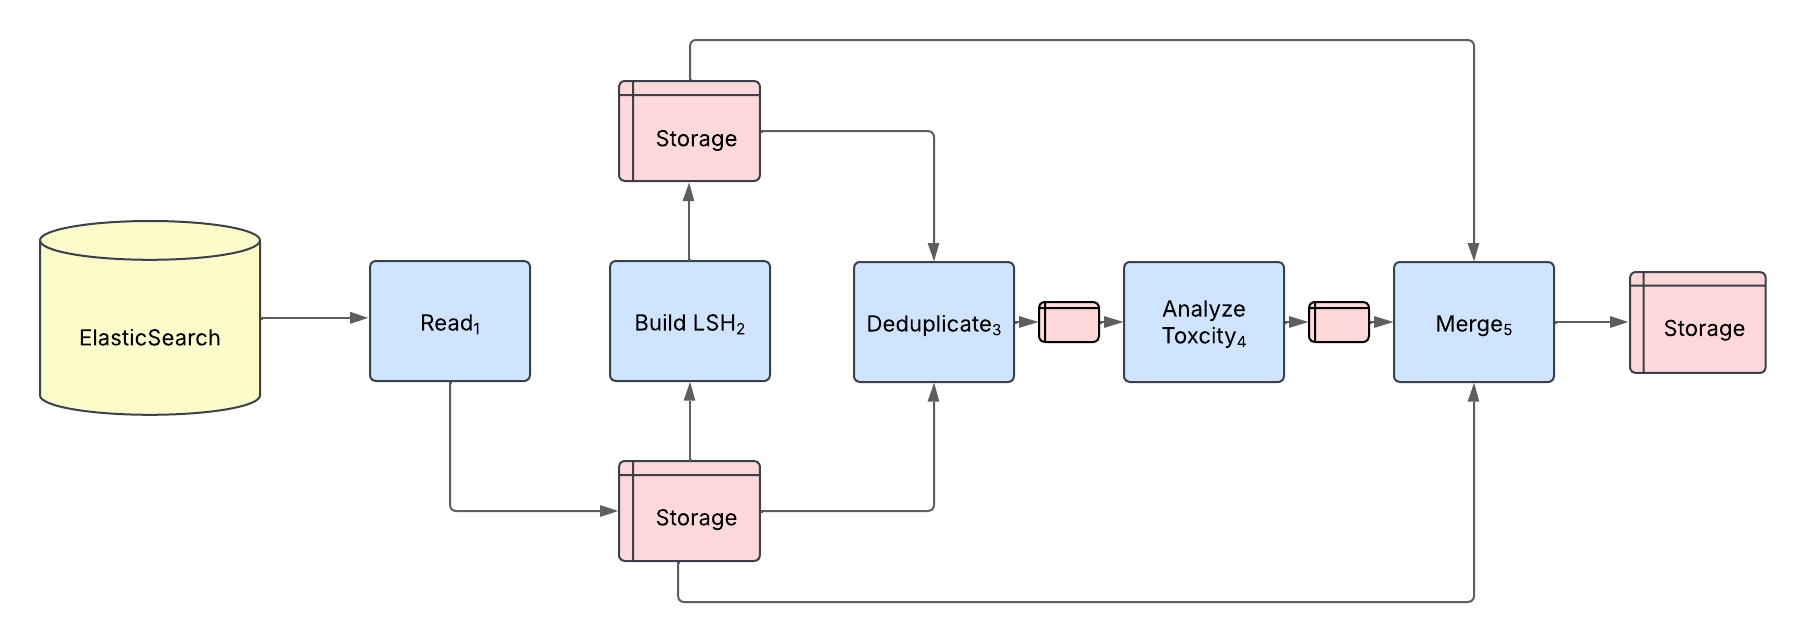
\includegraphics[width=\textwidth]{../material/pipeline.png}
    \caption{Data processing pipeline: 
    (\hyperref[step:ingestion]{1}) \textbf{Read \& Preprocess}: Reading data from the ElasticSearch database, extracting plaintext and calculating MinHash, then storing results; 
    (\hyperref[step:lsh]{2}) \textbf{Build LSH}: Building LSH index from processed data and storing it; 
    (\hyperref[step:dedup]{3}) \textbf{Deduplicate}: Near-duplicates are removed from processed data using the LSH index; 
    (\hyperref[step:toxicity]{4}) \textbf{Analyze Toxicity}: Performing toxicity analysis on deduplicated data; 
    (\hyperref[step:merge]{5}) \textbf{Merge}: Merging analyzed data with the original dataset using the LSH index. 
    Blue boxes represent processes, red indicates storage components, and yellow marks the external database.}
    \label{fig:pipeline}
\end{figure}

\section{LSH Index Construction and Toots Deduplication}\label{step:lsh_dedup} 
The deduplication stage employs Locality-Sensitive Hashing (LSH) techniques to efficiently identify and remove near-duplicate toots from the dataset. The idea of LSH is to group similar toots into buckets through a process called banding. This approach works by dividing each document's MinHash signature into $b$ bands of $r$ rows each. For a document with a MinHash signature of length $n$, we ensure $b \times r \le n$. Each band is then processed separately through a hash function, and toots sharing identical hash values in any band are considered potential duplicates. By setting the jaccard similarity threshold to 0.9, the optimizer finds values for $b$ and $r$ so that the probability of two toots sharing a band is very high when their Jaccard similarity is $\geq90\%$. The threshold is chosen to 0.9 because jaccard similarity is just indicating word similarity but not semantic similarity. Because we don't want to remove toots that are just similar in words but not in meaning, we choose a much higher threshold than the maybe more realistic threshold of 0.58 explored by \citet{wu:2020} for similarity in short texts.

\paragraph{LSH index construction}\label{step:lsh} The LSH index construction begins by reading the data from Parquet files generated in the previous processing stage. We just load two cloumns: the unique identifier (\textit{\_id}), and the precomputed MinHash values. These MinHash signatures are inserted into an LSH instance configured with our 0.9 similarity threshold. To optimize performance, we build multiple LSH instances in parallel using \textit{map\_batches}, then merge them into a single unified index. This merging is facilitated by Ray Actors, which provide stateful workers that maintain their internal state between operations. Unlike stateless functions, these actors allow us to incrementally build and combine LSH indexes while keeping memory usage manageable. The final consolidated LSH index is persisted as a pickle file for subsequent deduplication steps.

\paragraph{Deduplication}\label{step:dedup} During the deduplication phase, we now read three columns from the source Parquet files: the unique identifier (\textit{\_id}), the plaintext and the precomputed MinHash values. Additionally we load the prebuilt LSH index. For each toot we query the LSH index by inserting one minhash and receving all \textit{\_id}s in the same bucket. Those \textit{\_id}s belong to toots with Jaccard similarity of at least 90\%. Within each group of near-duplicates, we retain only the toot with the smallest \textit{\_id} value, ensuring deterministic selection while removing duplicates. This approach guarantees that only one representative instance of each near-duplicate group remains in the final dataset. The deduplicated results are then written back to Parquet files for further analysis and processing.

\section{Toxicity Analysis using Transformer-based Models}\label{step:toxicity}
After deduplication, the next stage involves predicting the toxicity of the deduplicated toots. This is done using pre-trained models designed to detect toxic content in text. The toxicity prediction is done in two main steps: language detection, and predicting toxicity labels.

\paragraph{Transformer-based Models}
Modern toxicity detection systems rely on Transformer-based language models, which have revolutionized natural language processing through their ability to learn contextualized word representations. The Transformer architecture, introduced by \citet{vaswani:2017}, works differently than older systems: instead of processing words one after another, it looks at all words in a sentence simultaneously. This allows it to better understand how distant words relate to each other, which is very important for detecting toxicity where harmful meaning often appear from combinations of words across a message."

Building on this foundation, \citet{devlin:2019} proposed Bidirectional Encoder Representations from Transformers (BERT), which introduced two key innovations. First, BERT trains by hiding random words in a sentence (like filling in blanks) and predicting them using both left and right context. This differs from older models that could only use previous words. Second, BERT learns whether two sentences logically follow each other, helping it understand conversation flow. These innovations enable BERT to create deep bidirectional representations that can be fine-tuned for downstream tasks with minimal architectural changes. The three toxicity detection models used in this study all use Transformer architectures.

% - just trained english text
% - trained on the "Jigsaw Toxic Comment Classification Challenge" dataset
% - dataset is build from wikipedia comments
% - labels like in table 5.1 but without sexual explicit
% - transformer-based model bert-base-uncased
% - fine-tuned on the Jigsaw... dataset
% - during prediction, input text is tokenized and passed through the transformer model
% - output is a probability score for the labels

\textbf{Detoxify Original}\footnote{\url{https://huggingface.co/unitary/toxic-bert}} is trained on English text using the "Jigsaw Toxic Comment Classification Challenge" dataset, which comprises Wikipedia comments. The model predicts probability scores for toxicity labels, which include categories similar to those listed in Table~\ref{toxicity-categories}, but without the sexually explicit label. The model is based on the BERT-base-uncased transformer architecture and fine-tuned on the Jigsaw dataset. During prediction, the input text is tokenized and processed through the transformer model to generate the output scores \cite{detoxify:medium}.

% - just trained english text
% - trained on the "Jigsaw Unintended Bias in Toxicity Classification" dataset
% - dataset is build from "Civil Comments" comments
% - labels like in table 5.1
% - for the training there are additional labels for identities, to reduce bias between different groups
% - transformer-based model roberta-base
% - fine-tuned on the Jigsaw... dataset
% - during prediction, input text is tokenized and passed through the transformer model
% - output is a probability score for the labels

\textbf{Detoxify Unbiased}\footnote{\url{https://huggingface.co/unitary/unbiased-toxic-roberta}} also focuses on English text but is trained on the "Jigsaw Unintended Bias in Toxicity Classification" dataset. This dataset consists of comments from "Civil Comments" platform and includes additional labels for identities to reduce bias across different demographic groups. The labels align with those in Table~\ref{toxicity-categories}. The model employs the RoBERTa-base transformer architecture and is fine-tuned on the Jigsaw dataset. Like Detoxify Original, it tokenizes input text and processes it through the transformer model to produce probability scores for the labels \cite{detoxify:medium}.

% - trained with multiple languages
% - For languages where less forum data is available, they use machine translation to translate labeled English-language comments into the target language.
% - training dataset is build from  variety of sources, including comments from online forums such as Wikipedia and The New York Times
% - Each comment is tagged by 3-10 crowdsourced raters
% - labels like in table 5.1 
% - start by training multilingual BERT-based models on data from online forums
% - distill these models into single-language Convolutional Neural Networks (CNNs) for each supported language
% - output is a probability score for the labels

\textbf{Perspective API} supports multiple languages and addresses the challenge of limited forum data for some languages by using machine translation. Labeled English-language comments are translated into the target language to supplement training data. The training dataset is sourced from diverse platforms, including Wikipedia and The New York Times, with each comment annotated by 3--10 crowdsourced raters. The labels match those in Table~\ref{toxicity-categories}. The training process begins with multilingual BERT-based models trained on the dataset, which are then distilled into single-language Convolutional Neural Networks (CNNs) for each supported language. As well as the two Detoxify models, the Perspective API outputs probability scores for the toxicity labels \cite{lees:2022}.

\paragraph{Language Detection using FastText}
To ensure only English texts are processed, a language detection step is performed. While the initial query filters for English-labeled toots, many are mislabeled. This additional filtering is critical because the toxicity prediction models from unitary cannot handle other languages.
For language detection, the deduplicated data is read from the Parquet files, and each task loads the FastText\footnote{\url{https://huggingface.co/facebook/fasttext-language-identification}} model. The model predicts the language of each toot’s plaintext, retaining only those labeled as English for further analysis.
FastText is ideal for this task due to its use of subword information (character n-grams), which enables robust handling of informal language, misspellings, and slang common in social media texts. Its efficiency and accuracy in language detection ensure reliable filtering, even for short or noisy inputs \cite{joulin:2016}.

\paragraph{Toxicity Prediction}
For toxicity classification, the selected toxicity model is loaded. For Detoxify models, this involves loading a transformer pipeline with truncation and padding enabled. For the Perspective API, the Google API client is used to make requests. We had to add a delay to respect the API's rate limit of 50 requests per second. The toxicity labels are predicted for each toot, and the results are appended to the dataset. The final dataset, including toxicity labels, is written back to Parquet files.

\section{MinHash-based Similarity Merging}\label{step:merge}
The final stage of the pipeline merges the toxicity labels back into the original dataset, ensuring the toxicity information is available for all toots—not just the deduplicated subset. The complete dataset is read from the Parquet files generated during the data reading stage. For each toot’s plaintext, the MinHash is computed, and the LSH index is queried to find similar toots. The smallest \textit{\_id} in the query results matches an \textit{\_id} in the deduplicated dataset. The toxicity labels corresponding to this \textit{\_id} are then concatenated with the queried toot. Finally, the toot, now containing all relevant information, is added to the final dataset, which is written back to Parquet files for further analysis.